\documentclass[tikz,border=4pt]{standalone}
\usepackage[T1]{fontenc}
\usepackage{mathptmx}
\usetikzlibrary{arrows.meta,calc}
\begin{document}
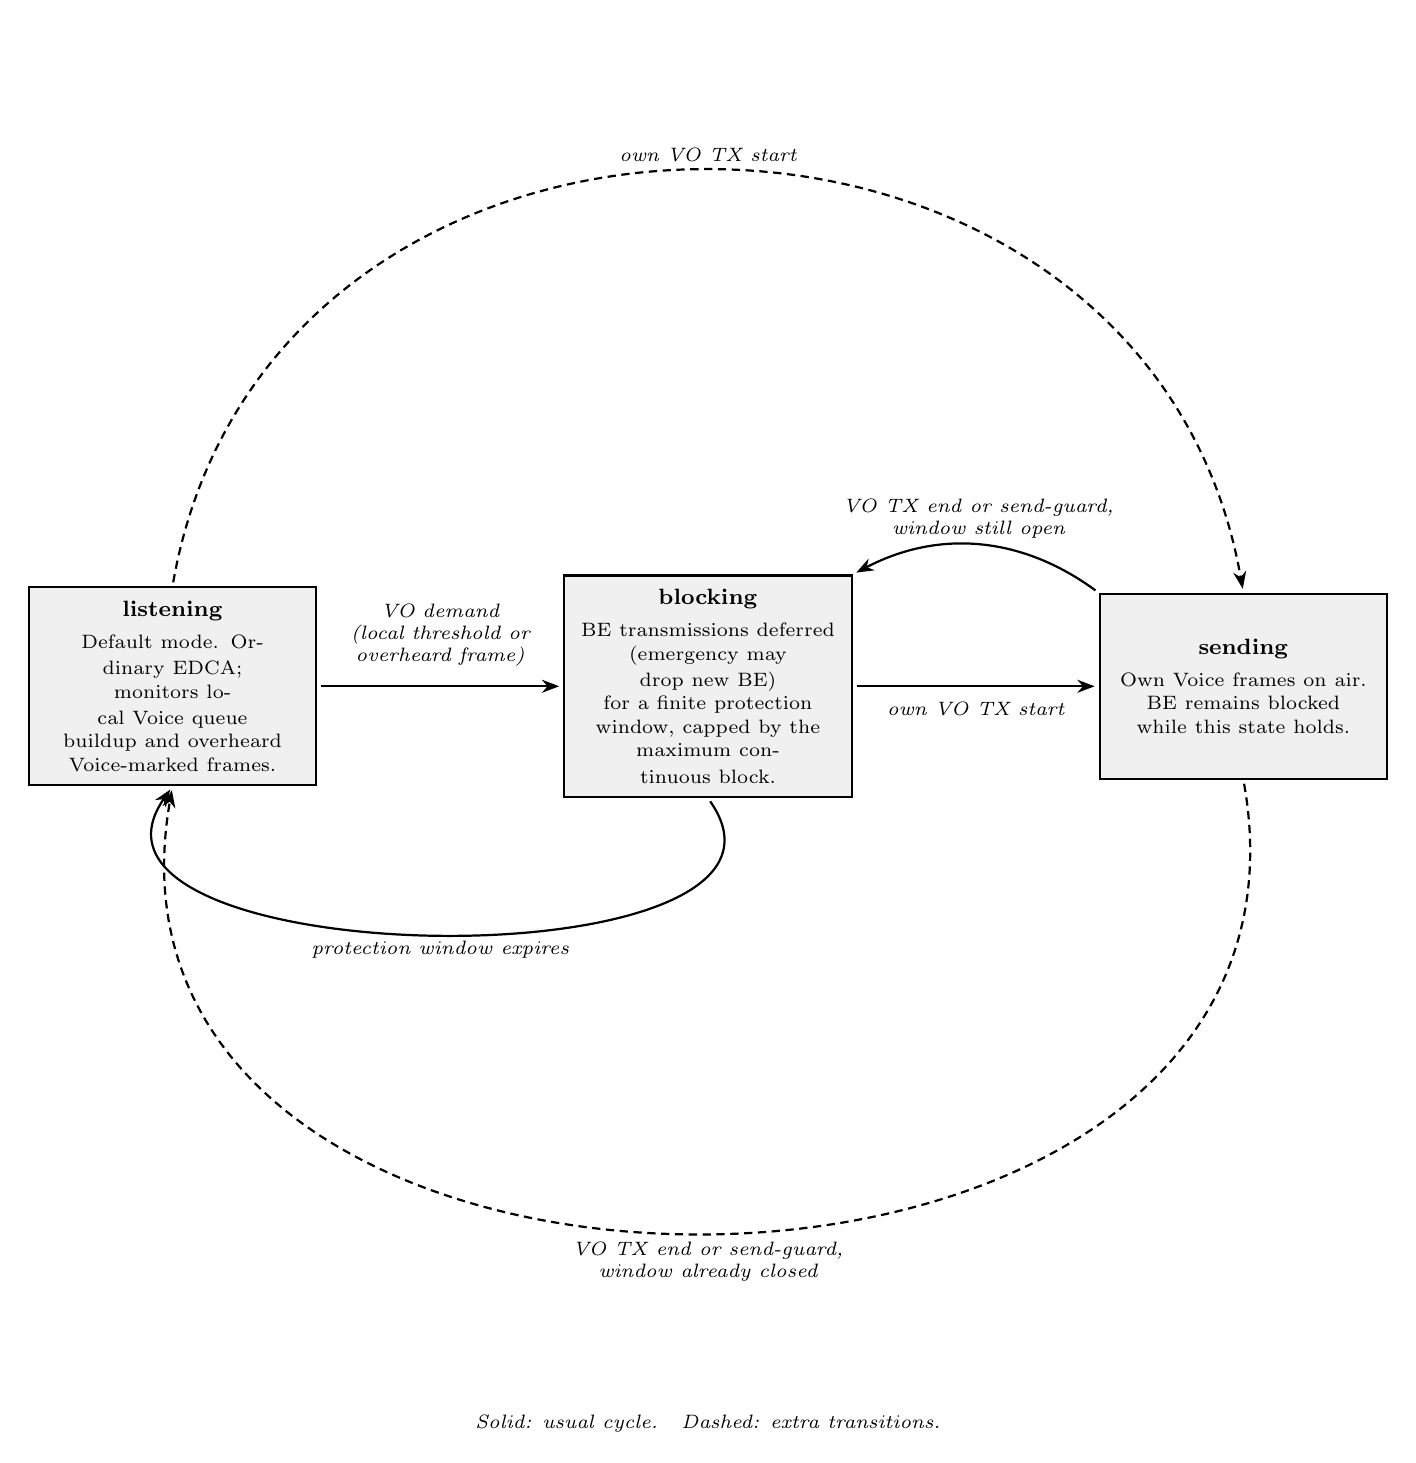
\begin{tikzpicture}[
  font=\footnotesize,
  >=Stealth,
  thick,
  state/.style={draw, thick, align=center, inner sep=5pt,
                text width=3.30cm, minimum height=2.35cm, fill=black!6},
  lbl/.style={font=\scriptsize\itshape, align=center, inner sep=1pt},
  arr/.style={-{Stealth[length=2.2mm]}, thick, shorten >=1.4pt, shorten <=1.4pt},
]
  \node[state] (lis) at (0.00,0.00) {%
    \textbf{listening}\\[2pt]
    {\scriptsize Default mode. Ordinary EDCA;}\\[-1pt]
    {\scriptsize monitors local Voice queue}\\[-1pt]
    {\scriptsize buildup and overheard}\\[-1pt]
    {\scriptsize Voice-marked frames.}};

  \node[state] (blk) at (6.80,0.00) {%
    \textbf{blocking}\\[2pt]
    {\scriptsize BE transmissions deferred}\\[-1pt]
    {\scriptsize (emergency may drop new BE)}\\[-1pt]
    {\scriptsize for a finite protection}\\[-1pt]
    {\scriptsize window, capped by the}\\[-1pt]
    {\scriptsize maximum continuous block.}};

  \node[state] (snd) at (13.60,0.00) {%
    \textbf{sending}\\[2pt]
    {\scriptsize Own Voice frames on air.}\\[-1pt]
    {\scriptsize BE remains blocked}\\[-1pt]
    {\scriptsize while this state holds.}};

  % listening → blocking. Label is in the upper corridor, narrower than the
  % gap, so it cannot sit on a state border or on the return arc below.
  \draw[arr] (lis.east) -- (blk.west);
  \node[lbl, anchor=south, text width=2.55cm] at ($($(lis.east)!0.5!(blk.west)$)+(0,0.20)$)
    {VO demand\\(local threshold or overheard frame)};

  % blocking → sending
  \draw[arr] (blk.east) -- (snd.west);
  \node[lbl, anchor=north] at ($($(blk.east)!0.5!(snd.west)$)+(0,-0.16)$)
    {own VO TX start};

  % sending → blocking (TX end / guard, window still open)
  \draw[arr] (snd.north west) to[bend right=32]
    node[lbl, above, pos=0.5, yshift=1pt]
      {VO TX end or send-guard,\\window still open}
    (blk.north east);

  % blocking → listening (blockTimer)
  \draw[arr] (blk.south) to[out=-55, in=-125, looseness=1.10]
    node[lbl, below, pos=0.5, yshift=-1pt] {protection window expires}
    (lis.south);

  % Extra: listening → sending
  \draw[arr, densely dashed] (lis.north) to[out=80, in=100, looseness=1.35]
    node[lbl, above, pos=0.5, yshift=2pt] {own VO TX start}
    (snd.north);

  % Extra: sending → listening
  \draw[arr, densely dashed] (snd.south) to[out=-80, in=-100, looseness=1.45]
    node[lbl, below, pos=0.5, yshift=-2pt]
      {VO TX end or send-guard,\\window already closed}
    (lis.south);

  \node[lbl, anchor=north] at ([yshift=-0.32cm]current bounding box.south)
    {Solid: usual cycle.\quad Dashed: extra transitions.};
\end{tikzpicture}
\end{document}
